\documentclass[9pt]{IEEEtran}

\usepackage[english]{babel}
\usepackage{graphicx}
\usepackage{epstopdf}
\usepackage{fancyhdr}
\usepackage{amsmath}
\usepackage{amsthm}
\usepackage{amssymb}
\usepackage{url}
\usepackage{array}
\usepackage{textcomp}
\usepackage{listings}
\usepackage{hyperref}
\usepackage{xcolor}
\usepackage{colortbl}
\usepackage{float}
\usepackage{gensymb}
\usepackage{longtable}
\usepackage{supertabular}
\usepackage{multicol}

\usepackage[utf8x]{inputenc}

\usepackage[T1]{fontenc}
\usepackage{lmodern}
\input{glyphtounicode}
\pdfgentounicode=1

\graphicspath{{./figures/}}
\DeclareGraphicsExtensions{.pdf,.png,.jpg,.eps}

\title{\vspace{0ex}
Long-Term Tracking with SiamFC}

\author{Dino Džaferagić\vspace{-4.0ex}}

\begin{document}

\maketitle

\section{Introduction}

This project studies long-term visual tracking. A short-term tracker assumes that the target stays visible. This fails when the target leaves the view or when the tracker drifts. I used SiamFC as the short-term base tracker. I then added a lost state and a re-detection step. The tracker uses the maximum raw correlation response as its confidence score.

\section{Method}

The base SiamFC tracker searches near the last target position. This works when the target moves in a smooth way. For long-term tracking, I mark the target as lost when the confidence score falls below a threshold. While lost, the tracker samples regions in the full image. It scores each region with the same SiamFC template. If the best score is above the threshold, the tracker returns to normal tracking.

I tested two sampling modes. Uniform sampling draws samples across the whole image. Gaussian sampling draws most samples near the last confident target position and adds a small number of uniform samples. The Gaussian spread grows while the tracker stays lost.

\section{Experiments}

I ran all tests on sequence \texttt{car9}. I used one sequence because the runs were done on a CPU. Table~\ref{tab:main} shows the main result. SiamFC-LT uses uniform sampling, 4 samples, and a re-detection threshold of 4.0. The long-term tracker gives a much higher recall because it can recover after drift.

\begin{table}[h]
    \centering
    \caption{Main result on \texttt{car9}.}
    \label{tab:main}
    \scriptsize
    \begin{tabular}{lccc}
        \hline
        Tracker   & Precision & Recall & F-score \\
        \hline
        SiamFC    & 0.639     & 0.271  & 0.381   \\
        SiamFC-LT & 0.602     & 0.596  & 0.599   \\
        \hline
    \end{tabular}
\end{table}

\subsection{Confidence Threshold}

The confidence score is the maximum raw value in the SiamFC correlation response. Table~\ref{tab:threshold} shows that a threshold that is too low delays re-detection. At threshold 3.5, the tracker stays in normal mode after it has drifted, so recall is low. Thresholds 4.0 and 4.5 work much better. In this sweep with 8 samples, threshold 4.5 gives the best F-score. However, the best tested full configuration was uniform sampling with 4 samples and threshold 4.0. Although threshold 4.5 gives the best F-score in this sweep, it also produces longer lost periods, which means that it is more conservative before returning to normal tracking.

\begin{table}[h]
    \centering
    \caption{Threshold sweep with 8 uniform samples.}
    \label{tab:threshold}
    \scriptsize
    \begin{tabular}{ccccc}
        \hline
        Threshold & Precision & Recall & F-score & Lost/event \\
        \hline
        3.5       & 0.592     & 0.268  & 0.369   & 11.21      \\
        4.0       & 0.601     & 0.589  & 0.595   & 2.29       \\
        4.5       & 0.602     & 0.590  & 0.596   & 29.00      \\
        \hline
    \end{tabular}
\end{table}

\subsection{Number of Samples}

Table~\ref{tab:samples} shows that more samples did not improve this sequence. On this sequence, 4 samples were already sufficient for the tested recovery events. More samples add more tests, but they do not change the final score much. All three settings recovered from each lost event in this run.

\begin{table}[h]
    \centering
    \caption{Uniform sampling with threshold 4.0.}
    \label{tab:samples}
    \scriptsize
    \begin{tabular}{ccccc}
        \hline
        Samples & Precision & Recall & F-score & Recovery rate \\
        \hline
        4       & 0.602     & 0.596  & 0.599   & 1.00          \\
        8       & 0.601     & 0.589  & 0.595   & 1.00          \\
        16      & 0.602     & 0.595  & 0.599   & 1.00          \\
        \hline
    \end{tabular}
\end{table}

\subsection{Sampling Type}

Table~\ref{tab:sampling} compares uniform and Gaussian sampling. Gaussian sampling gives a small gain on \texttt{car9}. It helps because the car often comes back near the last known area. The gain is small, so uniform sampling remains a good simple choice.

\begin{table}[h]
    \centering
    \caption{Sampling type with 8 samples and threshold 4.0.}
    \label{tab:sampling}
    \scriptsize
    \begin{tabular}{lccc}
        \hline
        Sampling & Precision & Recall & F-score \\
        \hline
        Uniform  & 0.601     & 0.589  & 0.595   \\
        Gaussian & 0.602     & 0.596  & 0.599   \\
        \hline
    \end{tabular}
\end{table}

\subsection{Re-detection Example}

Figure~\ref{fig:redetection} shows a lost frame and the later recovery. Green is ground truth, red is the tracker output, and cyan boxes are sampled regions. The tracker is lost at frame 789. It recovers at frame 808, after 19 frames. This example shows why the long-term mode improves recall: it stops trusting the local search and tests other image positions.

\begin{figure}[H]
    \centering
    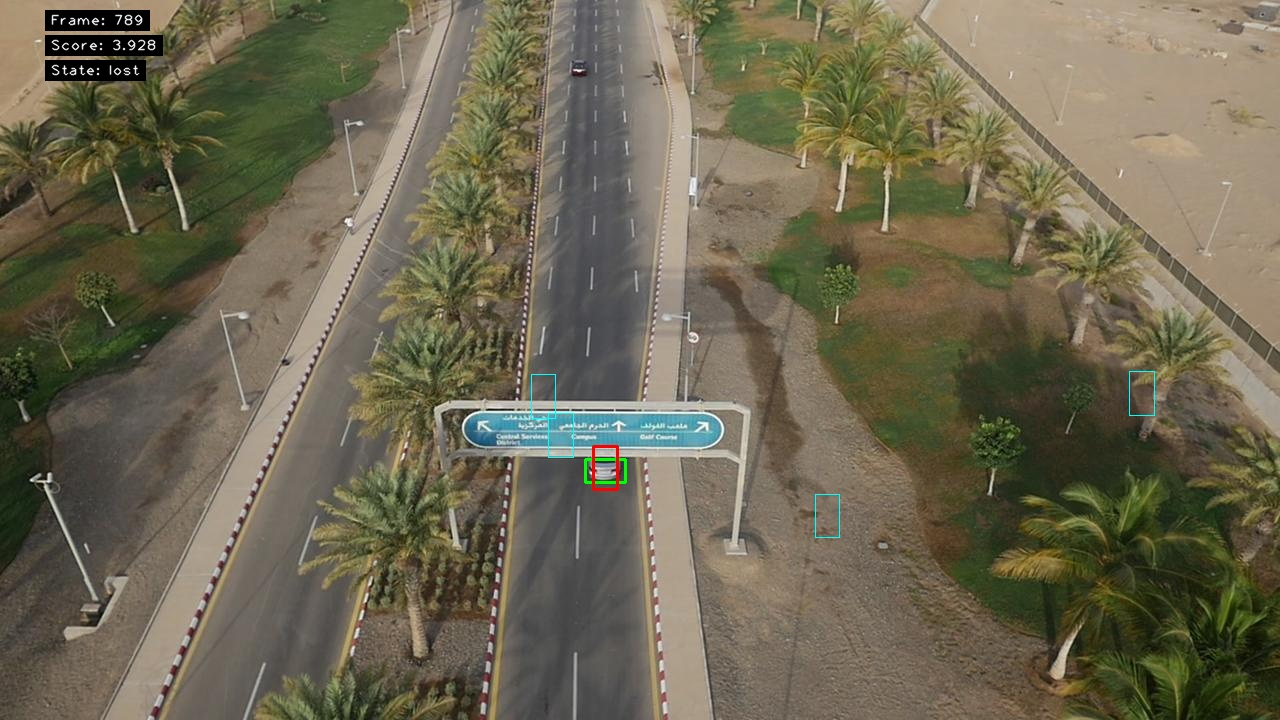
\includegraphics[width=0.50\columnwidth]{lost.jpg}

    \vspace{0.3ex}

    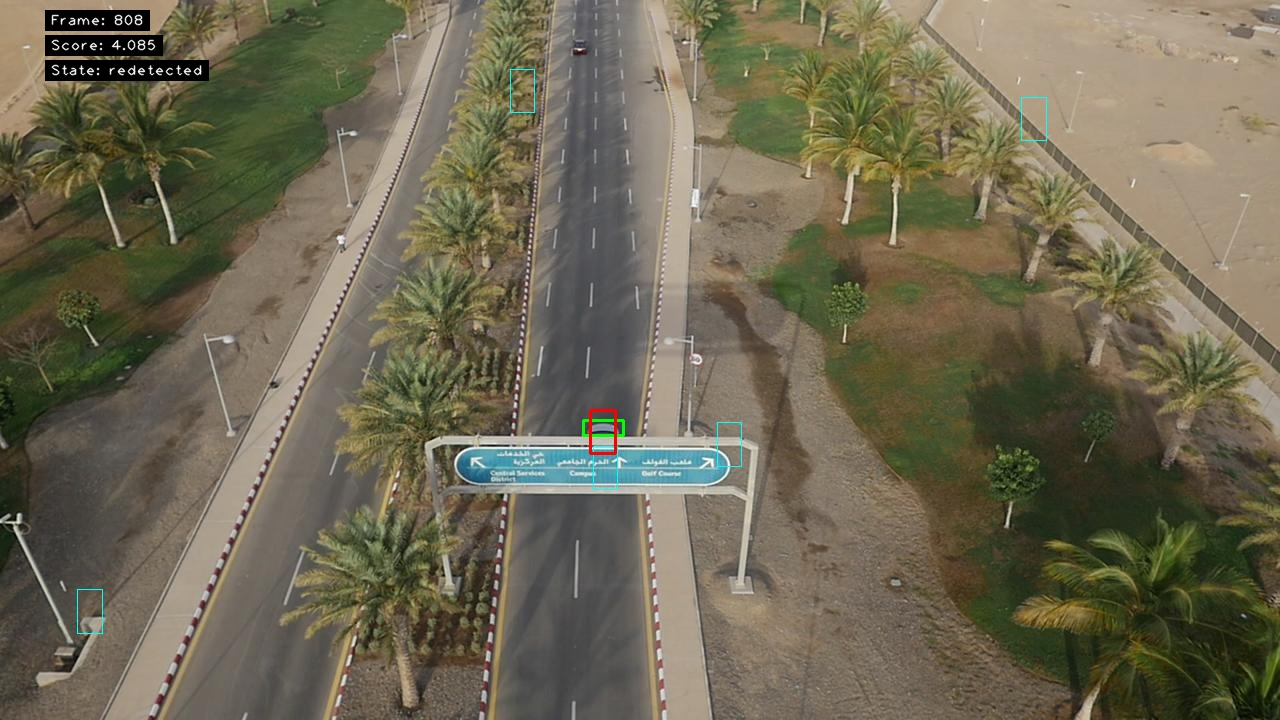
\includegraphics[width=0.50\columnwidth]{recovered.jpg}
    \caption{Target re-detection on \texttt{car9}. Top: lost frame 789. Bottom: re-detected frame 808. Cyan boxes show sampled regions during re-detection.}
    \label{fig:redetection}
\end{figure}

\section{Conclusion}

SiamFC-LT improves long-term tracking by detecting failure and searching the full image. On car9, the F-score increased from 0.381 to 0.599 as recall rose from 0.271 to 0.596. It can still miss the target when samples miss the right area or the response score is unclear.

\end{document}
